\section{Experiments: From Coalition Mechanism to Design Map}\label{sec:experiments}

The computational analysis is organized around a single question: when the physical network and aggregate demand are held fixed, when should routing authority be centralized and when should some independent decision centers be retained? We proceed from mechanism-isolating networks to a certified coalition-design policy. The bottleneck verifies the analytic regime threshold; Sioux Falls supplies a realistic benchmark for objective composition and governance-cost regimes; and independent Braess and grid topologies test whether the state transition and local merge policy survive a change in network geometry. Complete $n=4$ partition scans are used to measure policy regret, not as the scientific conclusion. Coalition partitions are counterfactual inputs throughout, so the experiments identify conditional equilibrium consequences rather than endogenous formation incentives.

\subsection{Experimental design and certification}\label{sec:experiment-design}

Every counterfactual keeps aggregate OD demand, physical link costs, and admissible routes fixed. In the identity-preserving treatment, each company retains its own accepted OD obligation, so a partition changes the aggregation of management objectives and the number of decision centers without changing the demand that must be served. The company-count scan holds total AV mass fixed while changing the number of underlying companies $n$; company HHI is reported descriptively and is not treated as a causal estimand. We report total system travel time (TSTT),
\begin{equation*}
 J(x)=\sum_{e\in E}x_ec_e(x_e),
\end{equation*}
and the normalized recovery $\rho$ in \eqref{eq:rho}. Because the user-equilibrium and system-optimum benchmarks are fixed within a comparison, maximizing recovery is equivalent to minimizing TSTT. Recovery is a normalized congestion-gap measure, not a percentage reduction in TSTT.

The finite-route variational inequality is solved with an adaptive Korpelevich extragradient method, simplex projection for each company--OD block, and player-specific shortest-path column generation. A profile is retained only when the normalized VI gap is at most $10^{-6}$ and the full-network omitted-route slack is at most $10^{-6}$ of the route-cost scale. The composition scan has $40$ certified rows with maximum VI gap $9.9998479\times10^{-7}$ and maximum relative omitted-route slack $9.9227901\times10^{-7}$; the degree scan has $54$ certified rows with corresponding maxima $9.9749371\times10^{-7}$ and $9.9064955\times10^{-7}$. The larger sensitivity, complete-partition, and pooling packages are certified under the same criteria.

\subsection{Mechanism tests: from scalar backfilling to screened responses}

\paragraph{Bottleneck.} Consider one affine congestible link $c_1(x_1)=t_0+t_1x_1$ and a constant alternative $c_2\equiv a$. On a fixed support, an interior coalition with perceived slope $\widehat\theta_C=\beta_Ct_1$ sends $b_C=(x^{UE}-x_1)/\beta_C$ on the bottleneck. Summing across responsive coalitions gives
\begin{equation}\label{eq:bottleneck-response}
 x_1=\frac{H+\Sigma x^{UE}}{1+\Sigma},
 \qquad
 \Sigma=\sum_{C\in D}\frac{1}{\beta_C},
\end{equation}
where $H$ collects HDV flow and coalition flow fixed at a corner. The equation makes the mechanism transparent: governance changes the aggregate coalition response through $\Sigma$, while HDV backfilling determines how much of that response reaches aggregate flow. For the canonical demand split, HDVs pin $x_1=x^{UE}$ below the support boundary $\alpha_c=1-x^{UE}/N$; above the boundary, the alternative HDV route leaves support and the coalition displacement becomes active. This is an exact scalar reduction, not a claim that general networks have a one-dimensional response.

\paragraph{Braess.} The Braess network uses demand $D=4000$, congested-edge cost $x_e/100$, outer-link costs $45$, a zero-cost shortcut, and three active fleet routes. The unrestricted route-space curvature is singular, but its restriction to OD-preserving directions is positive definite, so the projected coalition response is well defined. The response matrix has off-diagonal entries because changing one edge flow shifts mass across other edges used by the same OD routes. When all three HDV routes are active, the HDV tangent spans the coalition response and the activated operator is zero. Removing the shortcut from the HDV support removes one adjustment direction; the same coalition-side response then retains rank one. This pair of panels isolates the two transformations used in the theory: OD projection on the coalition side and HDV screening on the network side.

\begin{figure}[!htbp]
\centering
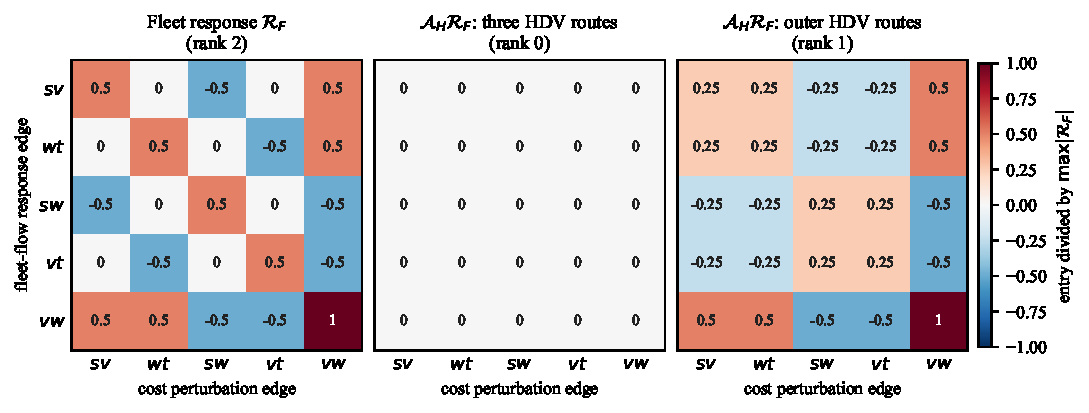
\includegraphics[width=\textwidth]{response_paper/figures/fig_braess_response_matrices.pdf}
\caption{Raw coalition response and HDV screening on the affine Braess network. Entries are normalized by the largest raw response entry. The coalition-side operator is held fixed across panels; changing only the HDV support changes the rank of the activated response.}
\label{fig:braess-response-matrices}
\end{figure}

\subsection{Sioux Falls: benchmarks and the conditional design criterion}

Sioux Falls has $76$ directed links and $528$ positive-demand OD pairs. The BPR benchmarks are $J^{UE}=7{,}480{,}226$ and $J^{SO}=7{,}194{,}256$, leaving a recoverable gap of $285{,}970$. Let $\mathfrak P(N)$ denote the set of partitions in the declared design menu and let $x^\ast(\Pi;\alpha,\gamma,\theta)$ be the certified continuation equilibrium under partition $\Pi$, AV penetration $\alpha$, coordination intensity $\gamma$, and objective-type vector $\theta$. The conditional design problem evaluated below is
\begin{equation}\label{eq:conditional-coalition-design}
 \Pi^\star(\alpha,\gamma,\theta)
 \in \arg\min_{\Pi\in\mathfrak P(N)}J\!\left(x^\ast(\Pi;\alpha,\gamma,\theta)\right).
\end{equation}
Equation~\eqref{eq:conditional-coalition-design} is an ex post design comparison over specified arrangements. It does not assign firms a payoff, permit deviations, or claim that the selected partition is stable.

\subsection{Objective composition at fixed concentration}\label{sec:sf-composition}

The first Sioux Falls experiment holds constant the quantities that a concentration statistic can see. Four equal-mass companies have objective types
\[
 (\tau_1,\tau_2,\tau_3,\tau_4)=(0.5,0.5,1.5,1.5),
\]
proportional but separately conserved OD obligations, company HHI $0.25$, two equal-mass coalitions, coalition HHI $0.5$, and identical route access. We compare assortative pairs $\{\{1,2\},\{3,4\}\}$ with mixed pairs $\{\{1,3\},\{2,4\}\}$. Only the composition of objective types within the coalitions changes.

\begin{table}[!htbp]
\centering
\small
\caption{Certified assortative-minus-mixed composition contrasts. Positive recovery differences favor assortative grouping; positive $\Delta J/J^{UE}$ means higher assortative TSTT.}
\label{tab:composition-contrast}
\begin{tabular}{ccrrrr}
\toprule
&&\multicolumn{2}{c}{$\alpha=0.5$}&\multicolumn{2}{c}{$\alpha=0.9$}\\
\cmidrule(lr){3-4}\cmidrule(lr){5-6}
$\gamma$&&$\Delta$ recovery (pp)&$\Delta J/J^{UE}$&$\Delta$ recovery (pp)&$\Delta J/J^{UE}$\\
\midrule
$0$    && $0.000$  & $0.0000\%$  & $0.000$  & $0.0000\%$\\
$0.25$ && $-0.294$ & $0.0112\%$  & $-1.285$ & $0.0491\%$\\
$0.50$ && $-1.168$ & $0.0446\%$  & $-1.161$ & $0.0444\%$\\
$0.75$ && $-0.244$ & $0.0093\%$  & $-0.228$ & $0.0087\%$\\
$1.00$ && $1.876$  & $-0.0717\%$ & $1.031$  & $-0.0394\%$\\
\bottomrule
\end{tabular}
\end{table}

At $\gamma=0$, the two partitions are invariant up to solver tolerance, as predicted by Proposition~\ref{prop:governance}. Once cross-member terms are active, the ordering changes with governance: mixed pairs close more of the recoverable gap at $\gamma=0.25$--$0.75$, whereas assortative pairs are better at $\gamma=1$. The largest baseline TSTT contrast is $0.0717\%$ of $J^{UE}$, so the effect is modest in absolute network time but decisive for the ordering of otherwise matched arrangements. This is a controlled identification result: an average objective type, coalition size, or HHI cannot recover the relevant response.

\begin{figure}[!htbp]
\centering
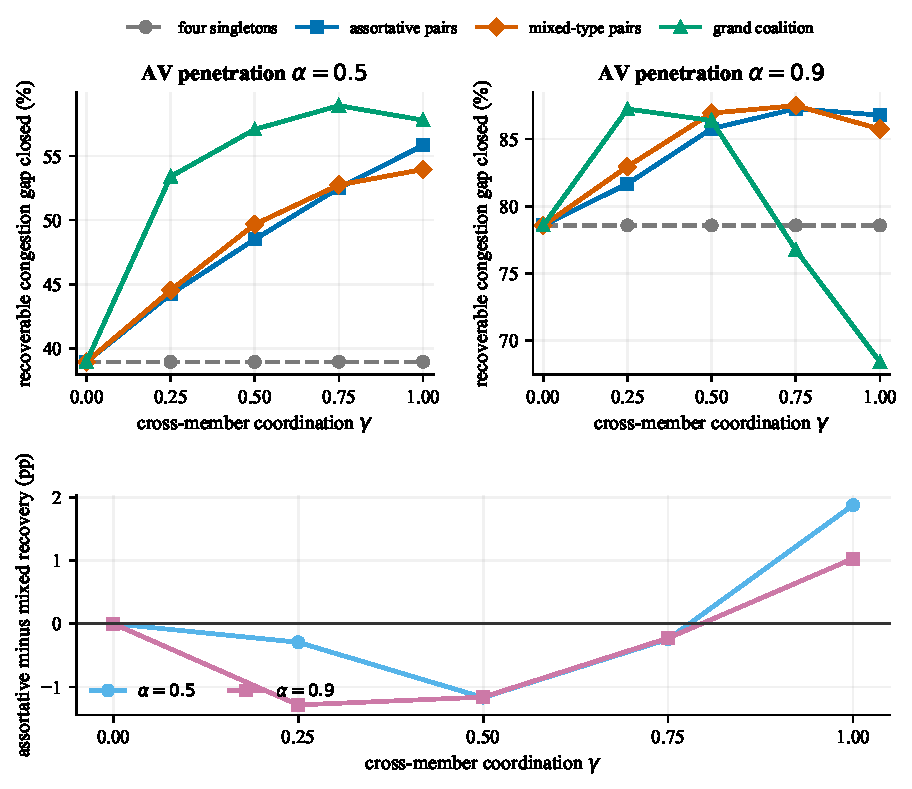
\includegraphics[width=\textwidth]{response_paper/figures/fig_sf_coalition_composition.pdf}
\caption{Coalition objective composition at fixed company masses, coalition sizes, OD obligations, and HHI. The top panels report recovery by partition; the bottom panel reports the assortative-minus-mixed recovery contrast.}
\label{fig:sf-composition}
\end{figure}

\subsection{State-contingent regimes in Sioux Falls}\label{sec:sf-design-map}

We evaluate all $15$ set partitions of the same four companies so that the
performance of any proposed selection rule can be measured against a known
benchmark. With $\varepsilon=10^{-8}$ in
\eqref{eq:epsilon-optimal-partitions}, Table~\ref{tab:best-partition} reports
the set of certified optima rather than forcing a numerical tie to be unique.

\begin{table}[!htbp]
\centering
\small
\caption{Set-valued optimum in the Sioux Falls $n=4$ audit scan. Company labels are one based. All comparisons use the same objective types, OD portfolios, route access, and identity-preserving governance rule.}
\label{tab:best-partition}
\begin{tabular}{ccp{5.0cm}rrr}
\toprule
$\alpha$ & $\gamma$ & $\varepsilon$-optimal partition set & $K$ & coalition HHI & gain vs. singleton (pp)\\
\midrule
0.5 & 0.5 & $\{\{1,2,3,4\}\}$ & 1 & 1.000 & 18.096\\
0.5 & 1.0 & $\{\{1,2,3,4\}\}$ & 1 & 1.000 & 18.810\\
0.9 & 0.5 & $\{\{1,2,3\}|\{4\},\ \{1,2,4\}|\{3\}\}$ & 2 & 0.625 & 8.745\\
0.9 & 1.0 & $\{\{1,2\}|\{3\}|\{4\}\}$ & 3 & 0.375 & 8.540\\
\bottomrule
\end{tabular}
\end{table}

The benchmark exhibits a clear state transition. At moderate AV penetration,
the grand coalition is optimal for both tested governance intensities. At high
penetration, partial coordination is optimal. The two three--one arrangements
at $\alpha=0.9,\gamma=0.5$ differ in TSTT by only $5.58\times10^{-7}$, or
$7.46\times10^{-12}J^{UE}$, because the two high-type companies are symmetric.
At $\gamma=1$, the optimum retains three decision centers. Thus stronger
governance does not imply that all companies should share one dispatcher. This
pattern is consistent with Theorem~\ref{thm:canonical-regimes}: coordination
should move the network toward its effective response target, which may lie at
an endpoint or in the interior.

\begin{figure}[!htbp]
\centering
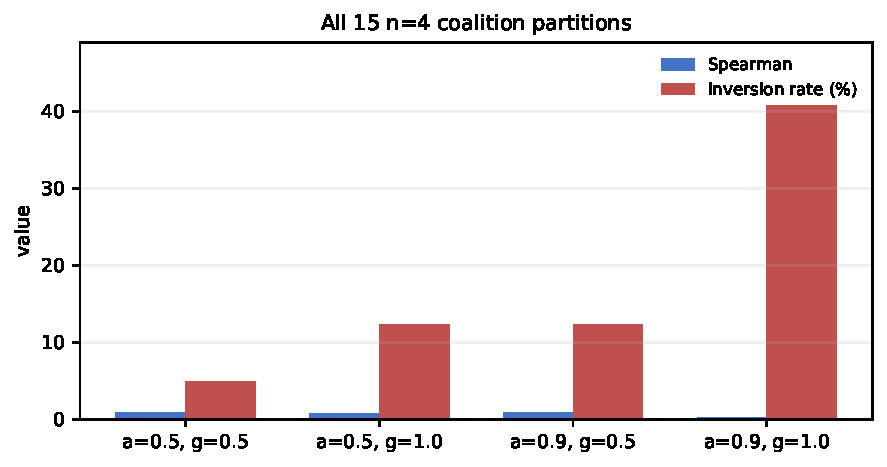
\includegraphics[width=0.9\textwidth]{response_paper/figures/fig_coalition_partition_scan.pdf}
\caption{Complete $n=4$ Sioux Falls audit scan. The exhaustive values establish the benchmark optimum used to evaluate local selection rules; they are not required by the rules themselves.}
\label{fig:coalition-partition-scan}
\end{figure}

\subsection{Local selection rules and policy regret}\label{sec:policy-regret}

For larger company sets, enumerating the Bell-number partition space is not a
practical design rule. We therefore test two agglomerative policies. The
one-step policy starts from singleton companies, evaluates every feasible
pairwise merge of the current blocks, chooses the best improving merge, and
stops when none improves TSTT. The two-step policy chooses the first merge on
the best improving path of length at most two. Both policies use only local
coarsenings of the current partition. The complete $n=4$ scans are retained
solely to calculate their ex post recovery regret
\begin{equation}\label{eq:policy-regret}
 \operatorname{Reg}(\widehat\Pi;s)
 :=100\frac{J(\widehat\Pi;s)-J^*(s)}{J^{UE}-J^{SO}}
 \quad\text{recovery percentage points}.
\end{equation}

\begin{table}[!htbp]
\centering
\small
\caption{Policy regret against the complete $n=4$ audit scans. Exact counts use the same relative TSTT tolerance as \eqref{eq:epsilon-optimal-partitions}.}
\label{tab:policy-regret}
\begin{tabular}{llrrr}
\toprule
benchmark & policy & exact states & mean regret (pp) & max regret (pp)\\
\midrule
Sioux Falls (4 states) & one-step merge & 4/4 & 0.000 & 0.000\\
 & two-step merge & 4/4 & 0.000 & 0.000\\
 & always grand & 2/4 & 4.908 & 18.695\\
 & always singleton & 0/4 & 13.548 & 18.810\\
\addlinespace
Braess and grid (32 states) & one-step merge & 29/32 & 0.332 & 8.339\\
 & two-step merge & 32/32 & 0.000 & 0.000\\
 & always grand & 27/32 & 1.520 & 18.205\\
 & always singleton & 0/32 & 21.752 & 42.289\\
\bottomrule
\end{tabular}
\end{table}

The one-step rule is exact in all Sioux Falls states and in $29$ of $32$
cross-network states, with mean regret $0.332$ points, but it has an $8.339$-point
failure on Braess at $\alpha=0.7,\gamma=0.75$. The other failures are $2.141$
points at $(0.9,0.5)$ and $0.130$ points at $(0.9,1)$. Two-step lookahead
repairs these local traps and reaches an $\varepsilon$-optimal arrangement in
all $36$ tested states. This is benchmark evidence, not a theorem of universal
optimality. For four companies the two-step neighborhood covers much of the
small partition lattice; for general $n$ it remains a local rule and avoids
requiring an ex ante enumeration of all Bell-number partitions.

\subsection{Governance-cost regimes}\label{sec:governance-cost-regimes}

The TSTT-minimizing organization need not be preferred once coordination
requires institutional resources. We apply \eqref{eq:penalized-coalition-loss}
to the Sioux Falls audit scan. At $\alpha=0.5,\gamma=1$, the lower envelope
passes through all four organizational degrees as $\lambda$ increases.

\begin{table}[!htbp]
\centering
\small
\caption{Governance-cost regimes at $\alpha=0.5,\gamma=1$. Endpoints are pairwise indifference thresholds; the displayed partition is optimal in the open interval.}
\label{tab:governance-regimes}
\begin{tabular}{lll r}
\toprule
$\lambda$ interval & selected partition & description & $K$\\
\midrule
$[0,0.0293)$ & $\{1,2,3,4\}$ & grand coalition & 1\\
$[0.0293,0.2678)$ & $\{1,2\}|\{3,4\}$ & two pairs & 2\\
$[0.2678,0.7435)$ & $\{1,2\}|\{3\}|\{4\}$ & one pair & 3\\
$[0.7435,\infty)$ & $\{1\}|\{2\}|\{3\}|\{4\}$ & singletons & 4\\
\bottomrule
\end{tabular}
\end{table}

The sequence is not imposed by a preference for intermediate structures. Each
partition supplies an equilibrium-congestion intercept and a governance-cost
slope; Proposition~\ref{prop:governance-cost-threshold} determines their
crossings. When coordination is inexpensive, the congestion gain justifies a
grand coalition. As the burden rises, partial coalitions retain the most
valuable internalization while avoiding some cross-company links. Fragmented
control becomes optimal only after the congestion benefit no longer covers the
governance burden.

\subsection{Cross-network validation of the regime transition}\label{sec:cross-network}

We repeat the complete $15$-partition audit on two independent BPR topologies:
a five-edge Braess network and a directed $3\times3$ grid with three ODs. The
design crosses four penetrations
$\alpha\in\{0.3,0.5,0.7,0.9\}$, four governance intensities
$\gamma\in\{0.25,0.5,0.75,1\}$, and the common objective vector
$(0.5,0.5,1.5,1.5)$. All $480=2\times4\times4\times15$ profiles pass the VI
and full-route oracle tests. The maximum VI gap is $9.971\times10^{-7}$ and
the maximum relative omitted-route slack is $3.79\times10^{-16}$.

\begin{table}[!htbp]
\centering
\small
\caption{Cross-network organizational regimes over 16 states per topology.}
\label{tab:cross-network-regimes}
\begin{tabular}{lrrl}
\toprule
network & grand-optimal states & partial-optimal states & transition at $\alpha=0.9$\\
\midrule
Braess & 14 & 2 & partial for $\gamma\in\{0.75,1\}$\\
directed grid & 13 & 3 & partial for $\gamma\in\{0.5,0.75,1\}$\\
\bottomrule
\end{tabular}
\end{table}

Both networks select the grand coalition in every tested state with
$\alpha\leq0.7$. At $\alpha=0.9$, sufficiently strong governance produces a
partial-coordination regime on both topologies, although the transition occurs
at a lower $\gamma$ on the grid. The qualitative state transition therefore
survives a change in topology, OD count, and cost calibration, while its
boundary remains network dependent.

\begin{figure}[!htbp]
\centering
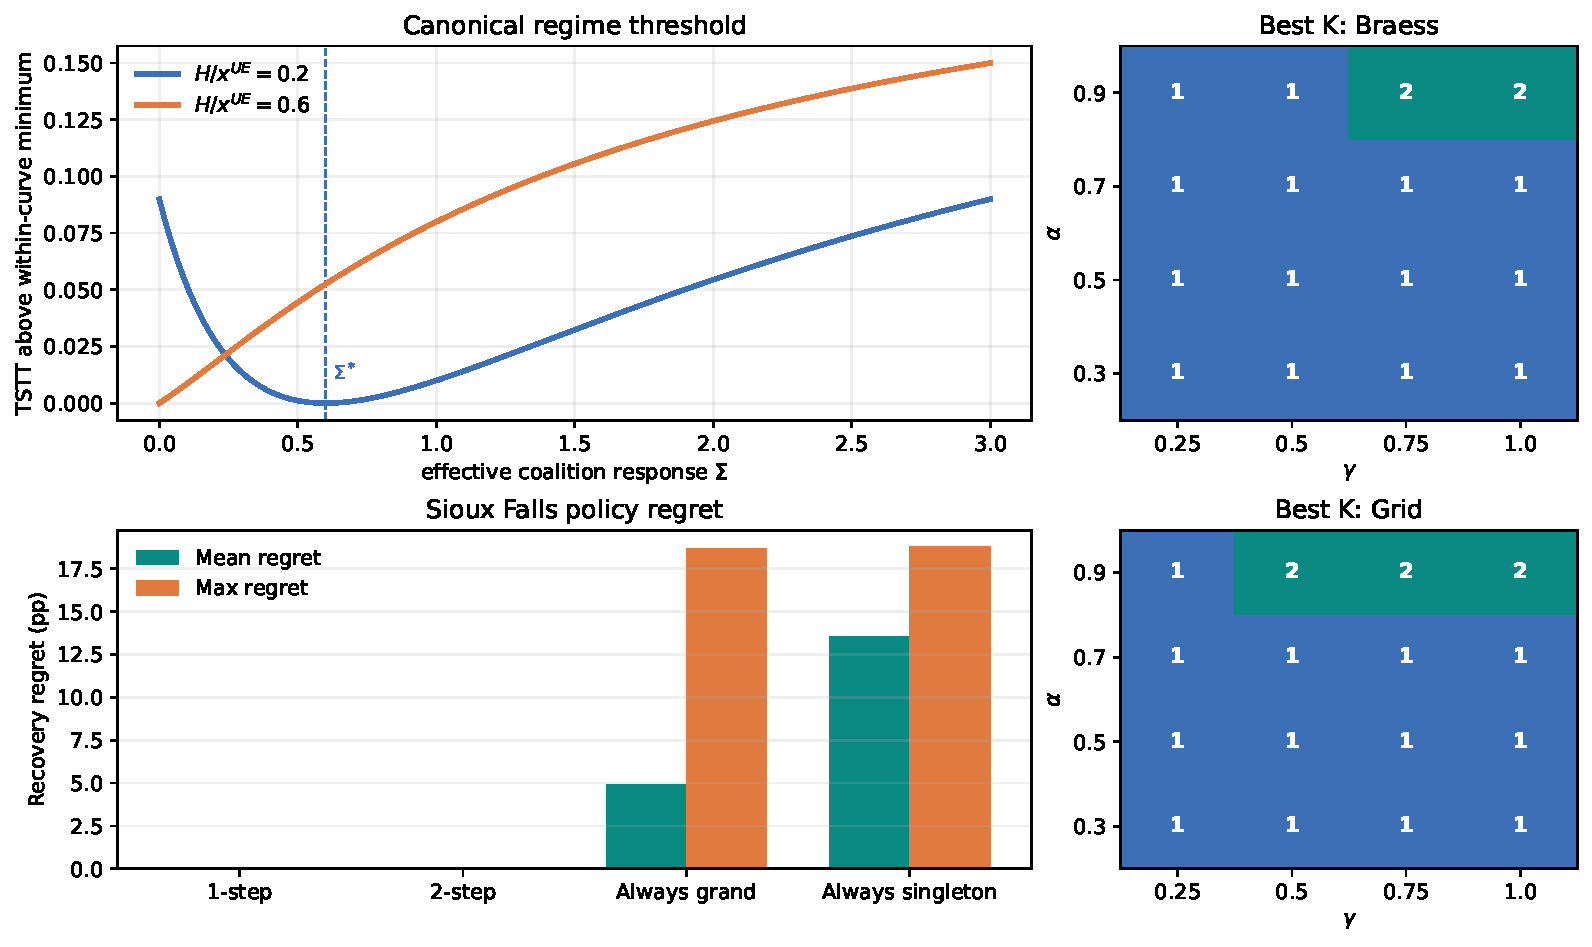
\includegraphics[width=\textwidth]{response_paper/figures/fig_regime_validation.pdf}
\caption{Regime theory and validation. The canonical bottleneck has an interior target $\Sigma^*$ only when $H<x^{UE}/2$; the Braess and grid heatmaps report the best coalition count; the Sioux Falls bars report policy regret.}
\label{fig:regime-validation}
\end{figure}

\subsection{Company count and coalition degree}\label{sec:sf-degree}

The degree scan varies the number of underlying companies $n\in\{2,4,8\}$ while holding total AV mass and aggregate demand fixed. Companies have equal mass within each $n$ and alternate low and high objective types. For each $n$, singleton, balanced intermediate, and grand-coalition partitions are compared within the same objective-type distribution.

\begin{table}[!htbp]
\centering
\small
\caption{Grand-minus-singleton coalition-degree effects at full cross-member coordination. Company HHI is descriptive; $K$ and $n$ are distinct organizational dimensions.}
\label{tab:degree-contrast}
\begin{tabular}{ccrrr}
\toprule
$\alpha$ & $n$ & $\rho_{K=1}-\rho_{K=n}$ (pp) & $\Delta J/J^{UE}$ & company HHI\\
\midrule
$0.5$ & $2$ & $1.956$ & $-0.075\%$ & $0.500$\\
$0.5$ & $4$ & $18.811$ & $-0.719\%$ & $0.250$\\
$0.5$ & $8$ & $29.489$ & $-1.127\%$ & $0.125$\\
$0.9$ & $2$ & $-18.365$ & $0.702\%$ & $0.500$\\
$0.9$ & $4$ & $-10.155$ & $0.388\%$ & $0.250$\\
$0.9$ & $8$ & $11.927$ & $-0.456\%$ & $0.125$\\
\bottomrule
\end{tabular}
\end{table}

At $\alpha=0.5$, the grand coalition improves recovery relative to singleton governance, with the effect increasing from $1.956$ to $29.489$ points as $n$ rises from $2$ to $8$. At $\alpha=0.9$, the same intervention is harmful for $n=2$ and $n=4$ but beneficial for $n=8$, ranging from $-18.365$ to $11.927$ points. Intermediate coordination is also material: at $\alpha=0.9$, moving from singletons to balanced pairs changes recovery by $7.179$ points for $n=4$ and $25.227$ points for $n=8$. The comparison makes clear why an ownership statistic cannot substitute for reporting both the underlying company count and the active coalition count.

\begin{figure}[!htbp]
\centering
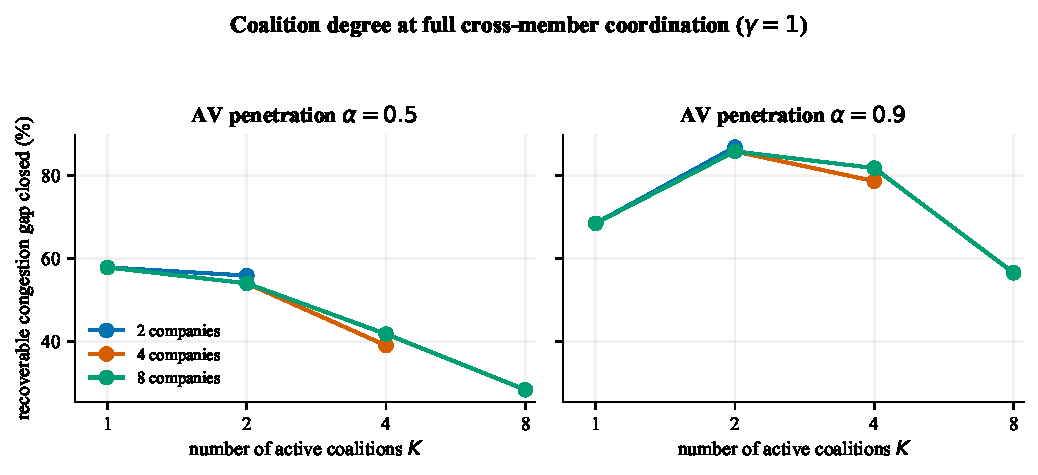
\includegraphics[width=0.95\textwidth]{response_paper/figures/fig_sf_coalition_degree.pdf}
\caption{Coalition degree at full cross-member coordination. Lines connect balanced partitions across the available coalition counts $K$ for each underlying company count $n$.}
\label{fig:sf-degree}
\end{figure}

\subsection{Sensitivity, audit diagnostics, and weak-effect boundaries}

The controlled composition comparison is repeated over objective-type gaps $\tau_H-\tau_L\in\{0.5,1.0,1.5\}$, reference management-slope scales $\{0.5,1,2\}\bar b$, five values of $\gamma$, and $\alpha\in\{0.5,0.9\}$. All $180$ profiles are certified. The two partitions coincide at $\gamma=0$ for every design. For $\gamma>0$, the contrast is generally nonzero but is not sign invariant. The absolute contrast reaches $9.089$ recovery points (wide gap, $\alpha=0.9$, unit slope scale). Sign reversals over $\gamma$ occur in multiple gap--scale combinations, including the baseline design. The robust statement is therefore behavioral: objective composition is active under coordination. No universal ranking of assortative and mixed grouping is supported.

\begin{table}[!htbp]
\centering
\small
\caption{Sensitivity summary for the assortative-minus-mixed recovery contrast. Each row aggregates five $\gamma$ values and is based on certified profiles.}
\label{tab:sensitivity-summary}
\begin{tabular}{cccrrr}
\toprule
$\alpha$ & type gap & slope scale & min contrast (pp) & max contrast (pp) & sign reversal\\
\midrule
0.5 & 0.5 & 0.5 & $-0.496$ & $0.210$ & yes\\
0.5 & 1.0 & 1.0 & $-1.168$ & $1.877$ & yes\\
0.5 & 1.5 & 1.0 & $-3.553$ & $0.000$ & no\\
0.9 & 0.5 & 1.0 & $-1.029$ & $0.018$ & yes\\
0.9 & 1.0 & 1.0 & $-1.285$ & $1.031$ & yes\\
0.9 & 1.5 & 1.0 & $-9.089$ & $0.000$ & no\\
\bottomrule
\end{tabular}
\end{table}

The complete $n=4$ scan also audits whether a mass statistic could substitute
for the response-based policy. All $15$ partitions are evaluated at
$\alpha\in\{0.5,0.9\}$ and $\gamma\in\{0.5,1\}$, yielding $60$ certified
profiles. At $\alpha=0.5$, coalition-HHI/recovery Spearman correlations are
$0.906$ and $0.793$ at $\gamma=0.5$ and $1$, with inversion rates $4.94\%$ and
$12.35\%$. At $\alpha=0.9$, the correlation falls from $0.815$ to $0.236$ and
the inversion rate rises from $12.35\%$ to $40.74\%$. The high-penetration,
full-coordination profiles span $0.684$--$0.871$ in recovery and $0.715\%$ of
$J^{UE}$ in TSTT. These are systematic within-benchmark diagnostics, not
population estimates. They explain why HHI is inadequate for selecting among
the candidate merges evaluated by the local policies.

\begin{table}[!htbp]
\centering
\small
\caption{All $n=4$ set-partition scan. Values are computed across the $15$ partitions in each condition.}
\label{tab:partition-scan}
\begin{tabular}{ccrrrr}
\toprule
$\alpha$ & $\gamma$ & Spearman & Kendall & inversion rate & recovery range\\
\midrule
0.5 & 0.5 & 0.906 & 0.807 & 4.94\% & $0.390$--$0.571$\\
0.5 & 1.0 & 0.793 & 0.671 & 12.35\% & $0.390$--$0.578$\\
0.9 & 0.5 & 0.815 & 0.671 & 12.35\% & $0.786$--$0.873$\\
0.9 & 1.0 & 0.236 & 0.165 & 40.74\% & $0.684$--$0.871$\\
\bottomrule
\end{tabular}
\end{table}

\begin{figure}[!htbp]
\centering
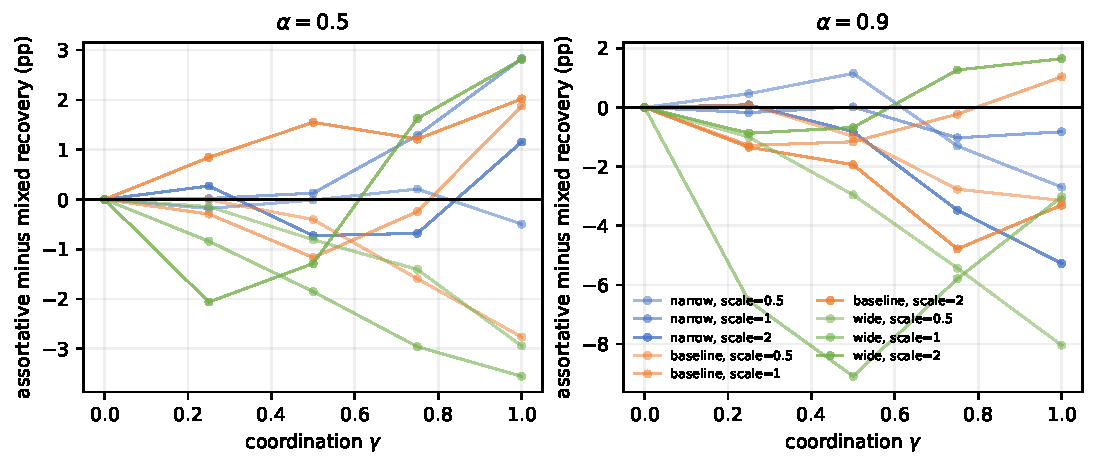
\includegraphics[width=\textwidth]{response_paper/figures/fig_coalition_sensitivity.pdf}
\caption{Objective-gap and governance-scale sensitivity. Lines report the certified assortative-minus-mixed recovery contrast over $\gamma$; colors denote objective gap and line opacity denotes reference-slope scale.}
\label{fig:coalition-sensitivity}
\end{figure}

\subsection{Spatial exposure and HDV penetration}

The fixed-HHI spatial experiment assigns four equal fleets the same total OD demand and company HHI $0.25$ but changes their spatial OD portfolios. Recovery spans $30.75\%$--$42.44\%$ at $\alpha=0.5$ and $10.15\%$--$74.33\%$ at $\alpha=0.9$. The largest displacement from proportional allocation is $0.363\%$ and $2.360\%$ of $J^{UE}$, respectively. Spatial exposure is therefore a design input alongside coalition size: identical masses can have different activated responses because they control different OD corridors.

\begin{figure}[!htbp]
\centering
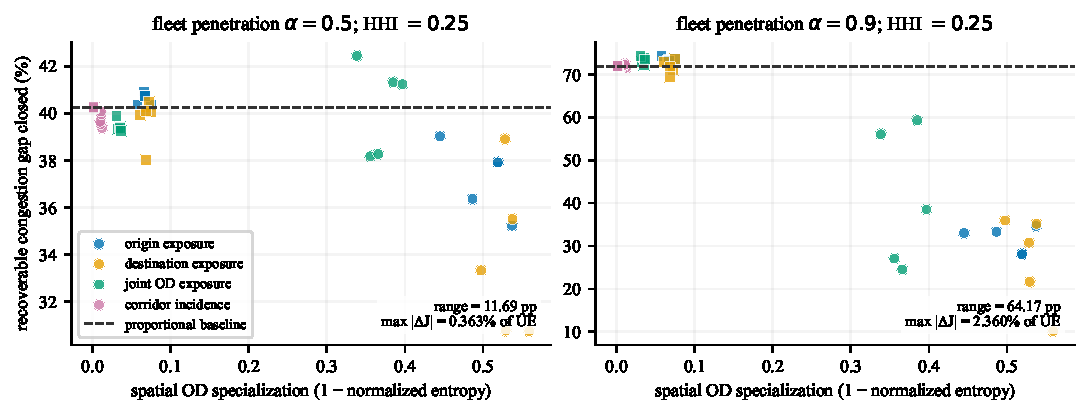
\includegraphics[width=\textwidth]{response_paper/figures/fig_sf_spatial_od.pdf}
\caption{Spatial OD portfolios change congestion at fixed equal fleet masses and HHI. The figure is a complementary exposure test, not a market-population estimate.}
\label{fig:sf-spatial}
\end{figure}

The penetration scan under common $\beta=1$ reports all-pair reversal rates of $18.10\%$, $18.73\%$, $10.65\%$, $10.14\%$, and $6.75\%$ at $\alpha=0.1,0.3,0.5,0.7,0.9$. Median reversal magnitudes range from $0.006\%$ to $0.043\%$ of $J^{UE}$. More HDVs can absorb a larger share of coalition displacement, reducing practical effect sizes; this transmission mechanism does not impose an ownership or coalition ordering. The earlier $200$-profile decomposition scan remains a robustness check: HHI--recovery Spearman correlations are $0.967$, $0.975$, and $0.988$ under the mass-linked prior, full-information $\beta=1$, and common $\beta=0.5$ regimes, with all-pair reversal rates $7.97\%$, $7.05\%$, and $4.14\%$. These proportional-portfolio results are secondary to the regime and policy analysis.

\subsection{Identity-preserving coordination versus operational pooling}

Pooling is a separate feasible-authority intervention, not another label for objective coordination. We compare the same two-coalition objective, company masses, aggregate OD demand, and $\gamma=1$ under identity-preserving and operational-pooling constraints. With proportional member OD portfolios and common route access, pooling changes member labels but not the induced aggregate route-flow set, as established in Proposition~\ref{prop:pooling}. Four certified profiles confirm the boundary: the largest pooling-minus-identity TSTT difference is $0.003$ time units, or $3.94\times10^{-10}J^{UE}$, and the largest recovery difference is $1.0308357\times10^{-6}$ percentage points. Pooling is neutral in this symmetric design. The result is a scope boundary, not evidence that pooling is neutral with heterogeneous route access or spatially specialized member portfolios.

\subsection{Summary of the evidence}

The experiments support a regime and policy conclusion rather than a universal
concentration law. Objective composition changes the coalition response only
when cross-member terms are active; OD portfolios and route geometry determine
where that response points; and HDV support determines how much reaches
aggregate congestion. The analytic bottleneck threshold explains why either
centralized or partial governance can be preferred. The cross-network scans
show the same broad transition from grand to partial coordination as AV
penetration and governance intensity rise, although the boundary is
topology-specific. A local one-step merge rule has low but nonzero regret, and
two-step lookahead reaches the audit optimum in all tested states. Governance
costs then generate explicit grand, partial, and fragmented intervals. The
result is a falsifiable selection framework for specified arrangements, not a
claim that firms will voluntarily form the selected coalition.
